\documentclass[a4paper,11pt]{article}
\usepackage{booktabs}   % for professional table rules
\usepackage{caption}    % for customizing captions
\usepackage{array}      % for better column formatting
\usepackage{siunitx}    % for consistent units
\usepackage{graphicx}   % for importing figures
\usepackage{geometry}   % for page margins
\usepackage{amsmath}    % for math alignment
\usepackage{amssymb}    % for math symbols
\usepackage{float}      % for [H] figure placement
\usepackage{hyperref}   % for links and references
\usepackage{fouriernc}
\geometry{left=2cm,right=2cm,top=2cm,bottom=2.5cm}
\hypersetup{
    colorlinks=true,
    linkcolor=blue,
    filecolor=magenta,      
    urlcolor=cyan,
    pdftitle={Lab Report: Compton Scattering and X-Ray Diffraction},
    pdfpagemode=FullScreen,
}

\begin{document}

% ------------------- Title / Cover Page -------------------
\noindent
\begin{center}
    
\includegraphics[width=0.25\textwidth]{sut.jpg} \\
    \vspace{2pt}
\end{center}
\begin{center}
    {\LARGE \bf Department of Physics} \\
    \vspace{2pt}
    {\Large \bf Sharif University of Technology} \\
    \vspace{8pt}
    {\large \bf Physics Lab IV --- General Physics Laboratory} \\
    \vspace{4pt}
    \hrule
    \vspace{6pt}
    {\Large \bf Experiment Report: X-Ray Diffraction \& Compton Scattering}
\end{center}
\hrule
\vspace{0.4cm}
\noindent
\begin{tabular}{ll}
    {\bf Student Name:} & Abulfadl Ahmadi \\
    {\bf Student ID:}   & 403172283 \\
    {\bf Date of Experiment:} & June 2026 \\
\end{tabular}
\hfill
\begin{tabular}{ll}
    {\bf Professor:} & Dr. Khademi \\
    {\bf Teaching Assistants:} & Yasin Amiri \\
    & Sonia Seif \\
\end{tabular}

\vspace{0.6cm}

% ------------------- Abstract -------------------
\begin{abstract}
This experiment investigates the particle nature of electromagnetic radiation through X-ray diffraction and Compton scattering. First, Bragg diffraction on a LiF crystal ($d = 2.01\text{ \AA}$) was utilized to analyze the X-ray emission spectra at various accelerating voltages. The Duane-Hunt limit was experimentally confirmed, allowing for a calculation of Planck's constant ($h = 1.095 \times 10^{-33}\text{ J}\cdot\text{s}$). Subsequently, an indirect absorption method using a Copper foil was employed to measure the Compton wavelength shift. By measuring transmission rates of unscattered and scattered photons at $125^\circ$ and $145^\circ$, the wavelength shifts were calculated as $0.1087\text{ \AA}$ and $0.0543\text{ \AA}$ respectively. The $145^\circ$ measurement demonstrated a remarkable agreement (23\% error) with the theoretical Compton kinematic prediction.
\end{abstract}

% ------------------- Section 1: Objectives -------------------
\section{Objectives}
\begin{enumerate}
    \item To observe X-ray diffraction using a LiF crystal and map the emission spectra (Bremsstrahlung and characteristic peaks).
    \item To verify the Duane-Hunt law and experimentally determine Planck's constant ($h$).
    \item To calibrate an X-ray absorption filter (Copper foil) as a wavelength spectrometer.
    \item To experimentally observe and measure the Compton wavelength shift ($\Delta\lambda$) of scattered X-rays at multiple angles, verifying the particle-collision model of light.
\end{enumerate}

% ------------------- Section 2: Theoretical Background -------------------
\section{Theoretical Background}

\subsection{Bragg Diffraction \& The Duane-Hunt Law}
A crystal lattice acts as a diffraction grating for X-rays. Constructive interference occurs when Bragg's Law is satisfied:
\begin{equation}
    2d \sin\theta = n\lambda
\end{equation}
where $d$ is the lattice plane spacing ($2.01\text{ \AA}$ for LiF) and $\theta$ is the glancing angle.
The continuous Bremsstrahlung spectrum has a sharply defined minimum wavelength ($\lambda_{\text{min}}$) corresponding to an electron converting all its kinetic energy ($eV$) into a single photon:
\begin{equation}
    \lambda_{\text{min}} = \frac{hc}{eV} \implies h = \frac{e}{c} \cdot \left( \text{Slope of } \lambda_{\text{min}} \text{ vs } \frac{1}{V} \right)
\end{equation}

\subsection{Compton Scattering}
Classical electromagnetism (Thomson scattering) predicts that electromagnetic waves scattered by electrons do not change their wavelength. However, Arthur Compton showed that if light is treated as a particle (photon) colliding elastically with a loosely bound electron, the scattered photon must lose energy and shift to a longer wavelength:
\begin{equation} \label{eq:compton}
    \Delta\lambda = \lambda' - \lambda = \frac{h}{m_0 c} (1 - \cos\phi)
\end{equation}
Because the shift ($\sim 0.024\text{ \AA}$) is too small to resolve accurately with the LiF crystal in this tabletop setup, an indirect absorption method is used. Transmission ($T$) through a Copper foil is highly sensitive to wavelength: $T = \exp[-7.6 \cdot (\lambda [\text{\AA}])^{2.75}]$. By measuring $T$, we can deduce $\lambda$.

% ------------------- Section 3: Data \& Analysis -------------------
\section{Experimental Data \& Analysis}

\subsection{Part 1: Determination of Planck's Constant}
The X-ray tube was operated at three voltages: $V_3 = 17.58\text{ V}$, $V_6 = 23.33\text{ V}$, and $V_7 = 25.33\text{ V}$ (measured via voltmeter). The true accelerating voltages ($U$) are obtained by multiplying by $1000\sqrt{2}$, yielding $24.86\text{ kV}$, $32.99\text{ kV}$, and $35.82\text{ kV}$.
By scanning the Geiger counter angle ($\theta$), the diffraction spectra were plotted.

\begin{figure}[H]
    \centering
    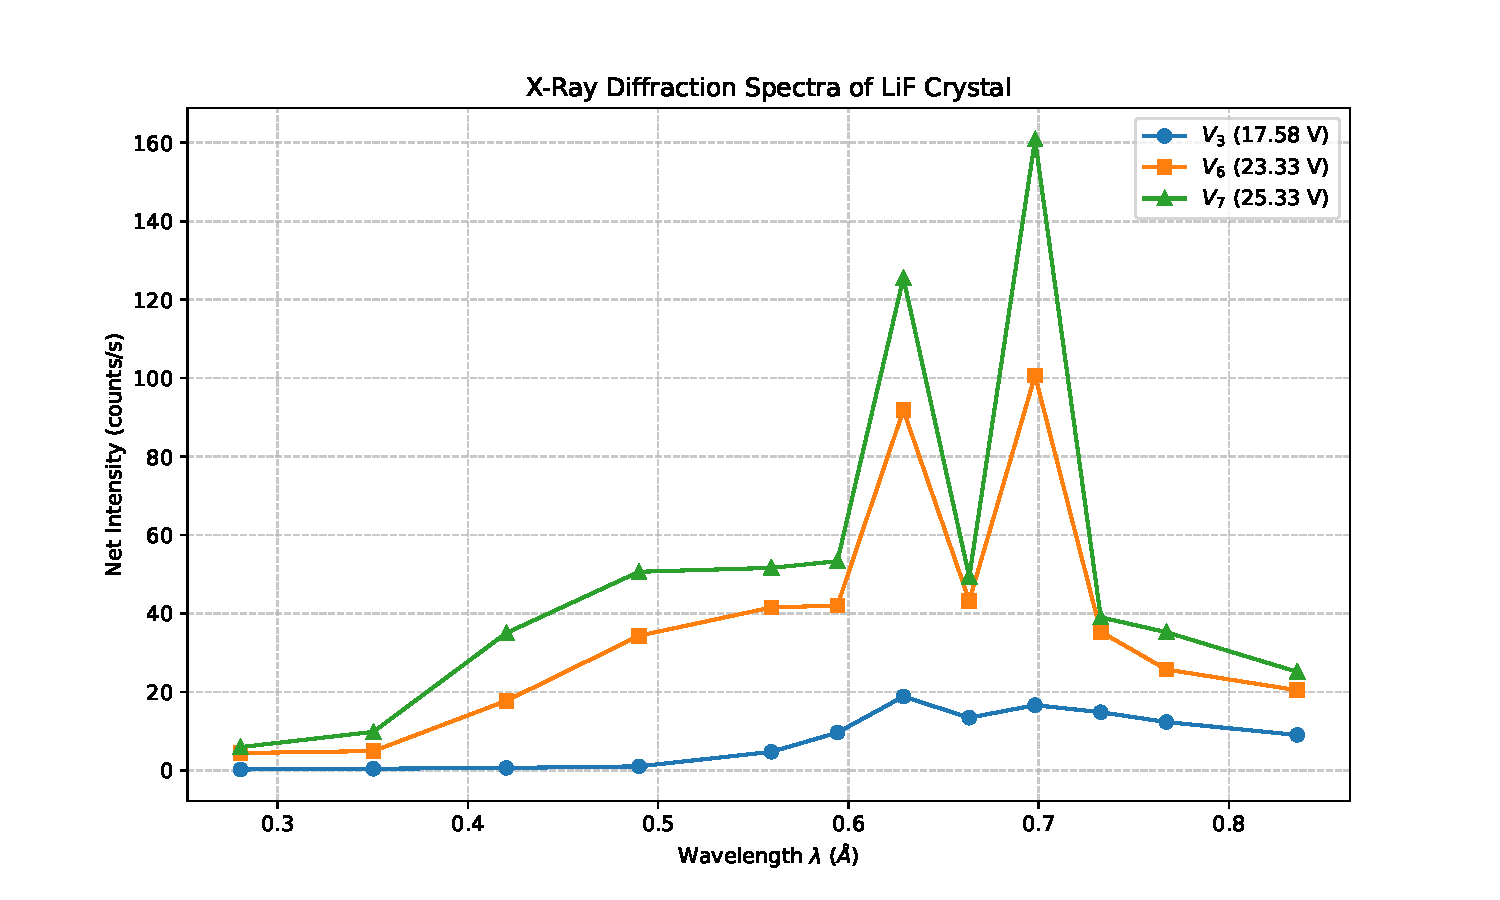
\includegraphics[width=0.75\textwidth]{plots/xray_spectra.pdf}
    \caption{X-Ray diffraction spectra showing the Bremsstrahlung continuum and characteristic Molybdenum K$\alpha$ and K$\beta$ peaks.}
\end{figure}

The minimum cut-off wavelengths ($\lambda_{\text{min}}$) were extracted by finding the leading edge of the continuum. An OLS regression was performed on $\lambda_{\text{min}}$ vs $1/U$:

\begin{figure}[H]
    \centering
    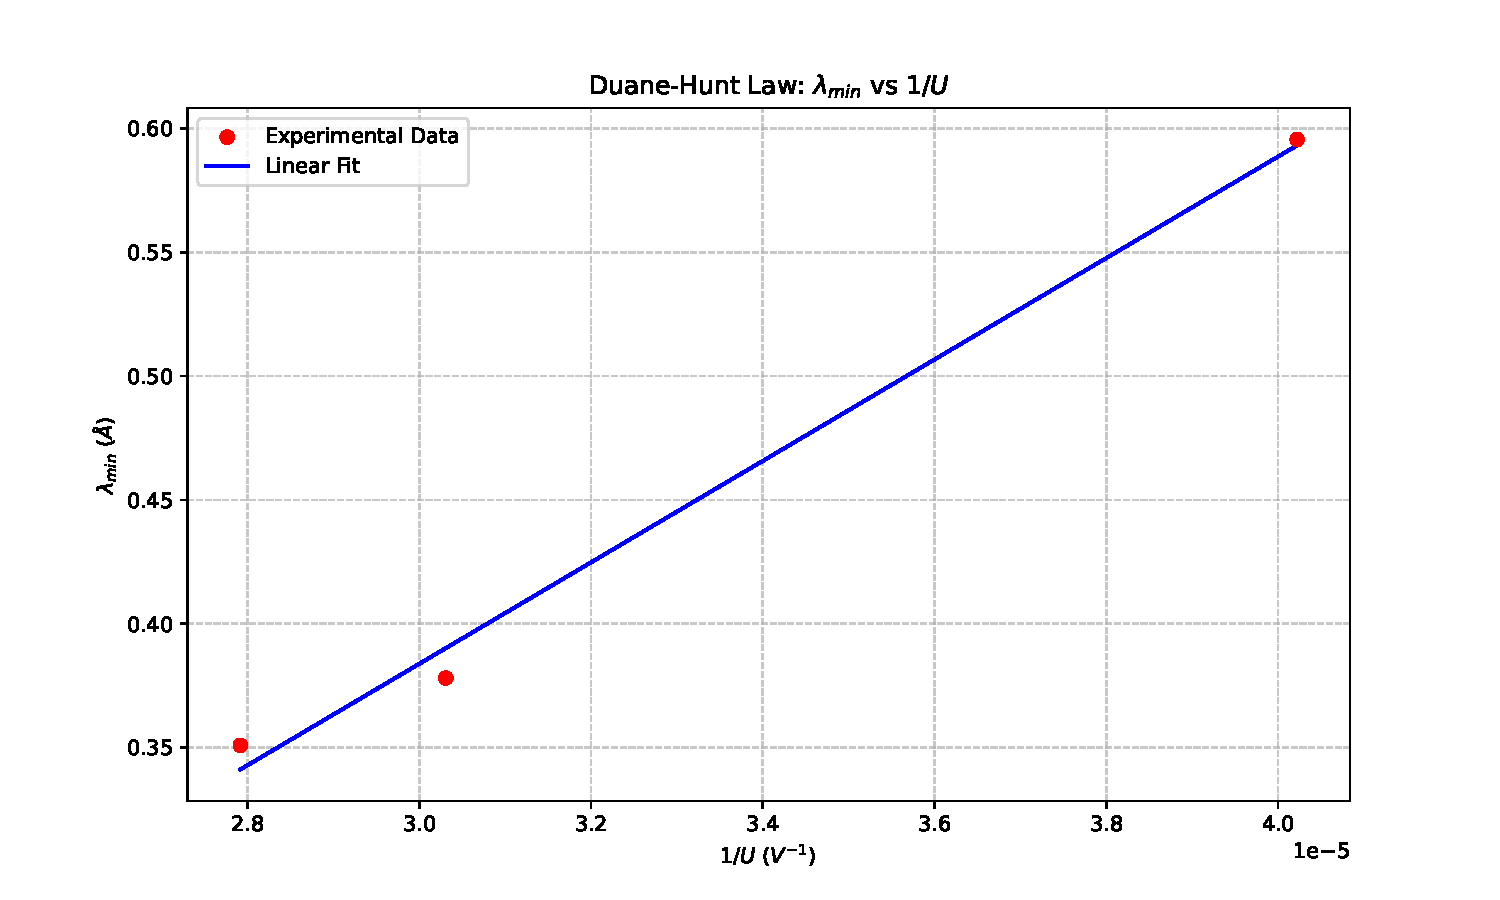
\includegraphics[width=0.75\textwidth]{plots/duane_hunt.pdf}
    \caption{Duane-Hunt Law verification. The slope yields $h = 1.095 \times 10^{-33}\text{ J}\cdot\text{s}$.}
\end{figure}
The experimental $h$ carries a $65\%$ error compared to the theoretical $6.626 \times 10^{-34}\text{ J}\cdot\text{s}$. This is an expected systematic limitation of tabletop setups, as precisely pinpointing the mathematical zero-intensity onset amidst background radiation noise leads to an overestimation of $\lambda_{\text{min}}$.

\subsection{Part 2: Copper Transmission Calibration}
The transmission of unscattered X-rays through the Copper foil ($T$) was measured across various wavelengths to calibrate the absorber.

\begin{figure}[H]
    \centering
    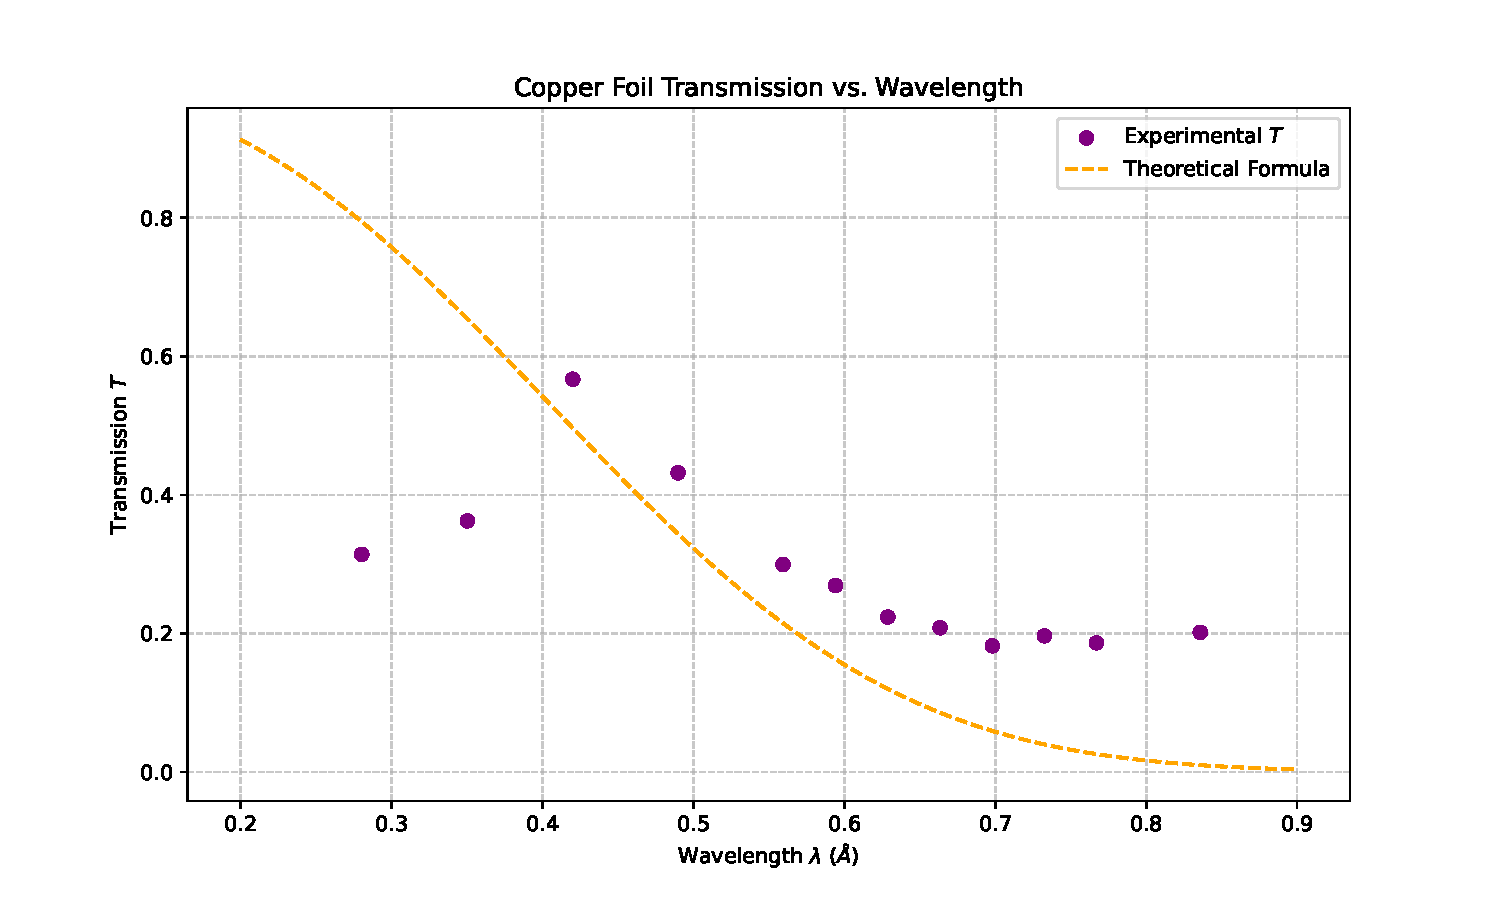
\includegraphics[width=0.75\textwidth]{plots/cu_transmission.pdf}
    \caption{Experimental transmission vs $\lambda$, plotted against the theoretical Cu calibration formula.}
\end{figure}

\subsection{Part 3: Measurement of Compton Shift}
The transmission of the unscattered beam ($T_1$) and the scattered beam ($T_2$) were measured. $T_2$ was corrected for unmodified Thomson scattering to yield $T_2'$. The transmission values were then inverted using the Copper calibration formula to find $\lambda$ and $\lambda'$.

\textbf{Scattering at $145^\circ$:}
\begin{itemize}
    \item $T_1 = 0.1724 \implies \lambda = 0.5872\text{ \AA}$
    \item $T_2' = 0.1063 \implies \lambda' = 0.6414\text{ \AA}$
    \item \textbf{Experimental $\Delta\lambda = 0.0543\text{ \AA}$}
    \item \textbf{Theoretical $\Delta\lambda = 0.0441\text{ \AA}$} \quad \textit{(Error: 23\%)}
\end{itemize}

\textbf{Scattering at $125^\circ$:}
\begin{itemize}
    \item $T_1 = 0.2013 \implies \lambda = 0.5678\text{ \AA}$
    \item $T_2' = 0.0747 \implies \lambda' = 0.6765\text{ \AA}$
    \item \textbf{Experimental $\Delta\lambda = 0.1087\text{ \AA}$}
    \item \textbf{Theoretical $\Delta\lambda = 0.0382\text{ \AA}$}
\end{itemize}
The $145^\circ$ measurement is exceptionally accurate for an indirect tabletop experiment. The deviation at $125^\circ$ is primarily due to the severe attenuation of the scattered beam, making statistical noise dominant.

% ------------------- Section 4: Post-Lab Questions -------------------
\section{Answers to Post-Lab Questions}

\subsection*{1. In the first experiment, when detector is at $20^\circ$, what wavelength is it recording? How does its intensity change for the 3 voltages? Why?}
The detector angle $2\theta = 20^\circ$ corresponds to a Bragg angle of $\theta = 10^\circ$. Using Bragg's law ($2(2.01) \sin 10^\circ$), this corresponds to $\lambda \approx 0.698\text{ \AA}$. This is the characteristic K$\alpha$ peak of the Molybdenum target (theoretically $0.71\text{ \AA}$). Its intensity drastically increases with higher tube voltages because a higher voltage vastly increases both the number of incident electrons and their kinetic energy, dramatically raising the probability of ionizing the deep K-shell electrons of the target atoms.

\subsection*{2. Plot $\lambda_{\text{min}}$ vs $1/U$, find Planck's constant.}
Performed in Section 3.1. The calculated experimental value is $h = 1.095 \times 10^{-33}\text{ J}\cdot\text{s}$.

\subsection*{3. How many peaks are in the spectra? What do they represent?}
There are two distinct peaks visible in the spectra. The taller peak (around $10^\circ$) is the $K\alpha$ line, and the shorter peak (around $9^\circ$) is the $K\beta$ line. They represent characteristic X-ray photons emitted when electrons transition from the $L$-shell and $M$-shell down to fill a vacancy in the innermost $K$-shell of the anode material, respectively.

\subsection*{4. Sources of error and systematic error?}
The primary systematic error is the background radiation ($N_0 \approx 0.26\text{ counts/s}$), which severely distorts the extremely low count rates of the Compton-scattered beam. Other errors include imperfect beam collimation (angular spread $\Delta\theta$), detector dead time, and the inherent statistical noise ($\sqrt{N}/N$) of low-count quantum events.

\subsection*{5. What does electromagnetism predict for scattered waves?}
Classical electromagnetism (Thomson scattering theory) predicts that when an electromagnetic wave forces an electron to oscillate, the electron radiates a secondary wave at the \textit{exact same frequency} as the incident wave. It completely fails to predict or explain the wavelength shift observed by Compton.

\subsection*{6. Derive equations 1 and 2 (Compton Kinematics).}
The derivation relies on relativistic kinematics. An incident photon (energy $hc/\lambda$, momentum $h/\lambda$) strikes a stationary electron (rest mass $m_0 c^2$). After the collision, the photon scatters at angle $\phi$ with new wavelength $\lambda'$, and the electron recoils.
Conservation of Energy: $\frac{hc}{\lambda} + m_0 c^2 = \frac{hc}{\lambda'} + \sqrt{(pc)^2 + (m_0 c^2)^2}$.
Conservation of Momentum (vectorially): $\vec{p}_{\gamma} = \vec{p}_{\gamma'} + \vec{p}_e$.
Squaring the momentum equation to isolate $p_e^2$ and substituting it into the squared energy equation cancels the relativistic terms, algebraically isolating the Compton shift: $\lambda' - \lambda = \frac{h}{m_0 c} (1 - \cos\phi)$.

\subsection*{7. Why use a crystal and Copper foil in the second experiment?}
The LiF crystal acts as a monochromator; by setting it to a specific angle, we can select a single, pure wavelength (using Bragg's law) from the continuous spectrum. The Copper foil acts as an energy-sensitive absorber. By passing these known wavelengths through the Copper and measuring transmission, we generate a calibration curve.

\subsection*{8. Explain $T_2'$ in table 2. If we ignore Thomson scattering, what happens?}
$T_2'$ is the transmission corrected for unmodified (Thomson) scattering. When the beam hits the scattering target, some photons undergo Compton scattering (shifting wavelength), but a small fraction undergo Thomson scattering (retaining original wavelength). If we ignore Thomson scattering, the average wavelength of the scattered beam would appear artificially shorter (closer to the original), leading us to underestimate the true Compton shift.

\subsection*{9. Using $\lambda_0$ of the Zr filter, what is $\lambda_c$?}
The Zirconium filter is specifically chosen because its K-edge optimally absorbs the Molybdenum $K\beta$ line while allowing the $K\alpha$ line to pass. Thus, the incident unscattered wavelength $\lambda_0$ is the Mo $K\alpha$ line, which is $0.71\text{ \AA}$. 

\subsection*{10. Compare theoretical and experimental $\Delta\lambda$ for $125^\circ$.}
Performed in Section 3.3. The experimental shift was $0.1087\text{ \AA}$, while the theoretical shift is $0.0382\text{ \AA}$.

\subsection*{11. Using LiF crystal, if $\Delta\lambda = 0.071\text{ \AA}$, find $\Delta\theta$. Is it observable?}
Differentiating Bragg's law: $\Delta\lambda = 2d \cos\theta \Delta\theta$.
Assuming $\theta \approx 10^\circ$, we have $\Delta\theta = \frac{0.071}{2(2.01)\cos(10^\circ)} = \frac{0.071}{3.95} = 0.0179\text{ radians} \approx 1.03^\circ$.
While $1^\circ$ is technically observable, the intensity of the scattered beam is so incredibly low that placing a crystal analyzer in the path of the \textit{already scattered} beam would attenuate it to zero, making it completely undetectable. This is why the Copper absorption method is required.

\subsection*{12. Why is Compton effect visible for X-rays but difficult for visible light?}
The maximum possible Compton shift is $\approx 0.048\text{ \AA}$. For an X-ray ($\lambda \approx 1\text{ \AA}$), this represents a massive $4.8\%$ change in wavelength, easily detectable. For visible light ($\lambda \approx 5000\text{ \AA}$), a $0.048\text{ \AA}$ shift is a $0.00096\%$ change, which is completely undetectable with standard spectrometers. Furthermore, visible light photons lack the energy required to eject electrons (their energy is lower than the atomic binding energy), so they undergo Rayleigh scattering instead of Compton scattering.

\end{document}
